
%(BEGIN_QUESTION)
% Copyright 2006, Tony R. Kuphaldt, released under the Creative Commons Attribution License (v 1.0)
% This means you may do almost anything with this work of mine, so long as you give me proper credit

%Magnetic flowmeters only function when measuring the flow of {\it electrically conductive} fluids.  First, explain why electrical conductivity is an essential property of the fluid.  Second, identify common fluids that {\it cannot} be detected by a magnetic flowmeter.  Third, determine whether slight changes in conductivity have any effect on the accuracy of a magnetic flowmeter (e.g. if the conductivity of the fluid decreased by a factor of two, would the output voltage similarly decrease by the same factor?).
Elektromagnetiske strømningsmålere fungerer bare med ledende v{\ae}sker. 
\begin{itemize}
\item{$\bullet$} Forklar hvorfor det er viktig at v{\ae}sken er ledende 
\item{$\bullet$} List noen vanlige v{\ae}sker som ikke kan brukes med elektromagnetiske flowmålere
\item{$\bullet$} Hvordan vil en økning av ledningsevne påvirke måleresultater (forutsatt at den i utgangspunktet leder godt nok)

\underbar{file i00523}
%(END_QUESTION)





%(BEGIN_ANSWER)

Answer to second question: most oils and concentrated alcohols have very low conductivity and thus cannot be measured by a magnetic flowmeter.  Gases and vapors suffer the same problem.

\vskip 10pt

In answer to the third question, I offer the following electrical ``thought experiment.''  Consider the effect of doubling the series resistance in this circuit:

$$\includegraphics[width=15.5cm]{i00523x01.eps}$$

\vskip 10pt

$$\includegraphics[width=15.5cm]{i00523x02.eps}$$

%(END_ANSWER)





%(BEGIN_NOTES)


%INDEX% Measurement, flow: magnetic

%(END_NOTES)


